% =============================================================================
\section{Binding Modules}
\label{sec:modules}
% =============================================================================
We describe the bindings generated by our system for various \cgal{}
packages and exemplify the use of the generated bindings.
%
When developing code in Python that uses the bindings, the statement
that imports the binding library, that is,
\begin{lstlisting}[style=pythonStyle]
>>> import CGALPY
\end{lstlisting}
must precede any statement that use the binding. This
statement is omitted in all examples hereafter.

% -----------------------------------------------------------------------------
\subsection{Two- and Three-Dimensional Kernel Bindings}
\label{ssec:modules:kernel}
% -----------------------------------------------------------------------------
The \iiDandiiiDGeometryKernelPackage{}
package~\cite{cgal:bfghhkps-lgk23-21a} of \cgal{} consists of
constant-size non-modifiable geometric primitive objects and
operations on these objects. The objects are sets of points in
$d$-dimensional affine Euclidean space, where $d = 2,3$.  Each point
is uniquely represented either by Cartesian coordinates or by
homogeneous coordinates. An object type can be defined either
precatively as a member of a kernel type or imperatively as a global
class-template parameterized by a kernel type, defined in the C++
\cppLstinline{CGAL} namespace. For example, assume that
\cppLstinline{Kernel} is a kernel type; the type that represents a
two-dimensional point of this kernel is either
\cppLstinline{Kernel::Point_2} or
\cppLstinline{CGAL::Point_2<Kernel>}.  We generate bindings only for
the latter types; that is, defining a two-dimensional point in Python
amounts to the code below.\footnote{When writing code in C++ the
  precative style is advantageous, as it enables the extension of
  kernel object types, which is irrelevant when generating bindings.}
\begin{lstlisting}[style=pythonStyle,basicstyle=\normalsize]
>>> Ker = CGALPY.Ker      # define the module namespace
>>> Point_2 = Ker.Point_2 # define the point type in the module namespace
>>> p = Point_2(0, 0);
\end{lstlisting}
Table~\ref{tab:ker} lists the \cmake{} flags associated with the
\iiDandiiiDGeometryKernelPackage{} module.  The kernel type is an
instance of a chain of C++ class templates. For convenience, \cgal{}
provides the following predefned types of generally useful kernels:
\begin{compactenum}
\item \cppLstinline{Exact\_predicates\_inexact\_constructions\_kernel}---provides exact geometric predicates, but geometric constructions may be inexact due to round-off errors.
  %
\item
  \cppLstinline{Exact\_predicates\_exact\_constructions\_kernel}---provides
  exact geometric constructions, in addition to exact geometric
  predicates.
  %
\item
  \cppLstinline{Exact\_predicates\_exact\_constructions\_kernel\_with\_sqrt}---same
  as \cppLstinline{Exact\_predicates\_exact \_constructions\_kernel},
  but the number type is a model of the concept that requires
  operations that perform square roots, namely
  \cppLstinline{FieldWithSqrt}.\footnote{See
    \url{https://doc.cgal.org/latest/Algebraic_foundations/classFieldWithSqrt.html}.}
  %
\item
  \cppLstinline{Exact\_predicates\_exact\_constructions\_kernel\_with\_kth\_root}---same as
  \cppLstinline{Exact\_predicates\_ exact\_constructions\_kernel}, but
  the number type is a model of the concept that requires operations
  that perform $k$-th roots, namely
  \cppLstinline{FieldWithKthRoot}.\footnote{See
    \url{https://doc.cgal.org/latest/Algebraic_foundations/classFieldWithKthRoot.html}}
  %
\item \cppLstinline{Exact\_predicates\_exact\_constructions\_kernel\_with\_root\_of}---same as
\cppLstinline{Exact\_predicates\_ exact\_constructions\_kernel}, but the number type is a model of the concept that requires operations that computes the root of univariate polynomial, namely \cppLstinline{FieldWithRootOf}.\footnote{See \url{https://doc.cgal.org/latest/Algebraic_foundations/classFieldWithRootOf.html}.}
\end{compactenum}

%%%%%%%% Kernel Module Flags
\begin{table}[!htp]
  \caption{\iiDandiiiDGeometryKernelPackage{} module flags}
  \centering\begin{tikzpicture}
  \matrix (first) [tableModuleFlags,
    column 1/.style={nodes={text width=17em}},
    column 2/.style={nodes={text width=3.5em}},
    column 3/.style={nodes={text width=4em}},
    column 4/.style={nodes={text width=23.5em}},
    row 3/.style={nodes={minimum height=2.8em}}
  ] {
    Name & Type & Default & Description\\
    \cmakeLstinline{KERNEL\_NAME} & String & \myLstinline{epic} &
      The kernel type used\\
    \cmakeLstinline{KERNEL\_INTERSECTION\_BINDINGS} & Boolean &
      \myLstinline{true} &
      Determines whether to generate bindings for intersections\\
  };
 \end{tikzpicture}
 \label{tab:ker}
\end{table}

All the predefined types are of Cartesian kernels. The \cmake{} flag \myLstinline{KERNEL\_NAME} specifies which kernel type should be used for the generated bindings.  Currently, only a limited predefined types and two specific types are supported; see Table~\ref{tab:ker:name}.

%%%%%%%% Kernel Name Options
\begin{table}[!htp]
  \caption{Kernel name options.}
  \centering\begin{tikzpicture}
    \matrix (first) [tableName,
      column 1/.style={nodes={text width=8em}},
      column 2/.style={nodes={text width=34em}}
    ] {
    \cmakeLstinline{KERNEL\_NAME} & Predefined Type\\
    \myLstinline{epic} &
      \cppLstinline{Exact\_predicates\_inexact\_constructions\_kernel}\\
    \myLstinline{epec} &
      \cppLstinline{Exact\_predicates\_exact\_constructions\_kernel}\\
    \myLstinline{epecws} &
      \cppLstinline{Exact\_predicates\_exact\_constructions\_kernel\_with\_sqrt}\\
   };
 \end{tikzpicture}
   \centering\begin{tikzpicture}
    \matrix (first) [tableName,
      row 2/.append style={nodes={minimum height=2.8em}},
      row 3/.append style={nodes={minimum height=2.8em}},
      column 1/.style={nodes={text width=19em}},
      column 2/.style={nodes={text width=23em}}
    ] {
    \cmakeLstinline{KERNEL\_NAME} & Predefined Type\\
    \myLstinline{filteredSimpleCartesianDouble} &
      \setlength{\tabcolsep}{0pt}\renewcommand{\arraystretch}{0}
      \begin{tabular}{l}
        \cppLstinline{NT = double}\\[5pt]
        \cppLstinline{Filtered\_kernel<Simple\_cartesian<NT>>}
      \end{tabular}\\
    \myLstinline{filteredSimpleCartesianLazyGmpq} &
      \setlength{\tabcolsep}{0pt}\renewcommand{\arraystretch}{0}
      \begin{tabular}{l}
        \cppLstinline{NT = Lazy\_exact\_nt<Gmpq>}\\[5pt]
        \cppLstinline{Filtered\_kernel<Simple\_cartesian<NT>>}
      \end{tabular}\\
   };
 \end{tikzpicture}
 \label{tab:ker:name}
\end{table}

The kernel type determines the underlying number type used to
represent coefficients and coordinates of kernel objects and for
evaluating mathematical expressions that involve these coefficients
and coordinates. The Python attribute \pyLstinline{FT}, nested in the
Python namespace \pyLstinline{Ker}, exposes the C++ underlying number
type when it is not a primitive data type; that is, when the selected
kernel is nor
\cppLstinline{Exact\_predicates\_inexact\_constructions\_kernel}
neither
\cppLstinline{Filtered\_kernel<Simple\_cartesian<double>>}. (In both
cases the underlying number type is \cppLstinline{double}.) Similar to
the Python code above, the code below defines a two-dimensional point;
here, the coordinates are explicitly converted to the underlying
number type.
\begin{lstlisting}[style=pythonStyle]
>>> p = Point_2(Ker.FT(0), Ker.FT(0))
\end{lstlisting}

The code excerpt shown in Listing~\ref{lst:cmake:epecFixed}, in the
\cmake{} language, sets the \cmake{} flags for our first example. When
\myLstinline{cmake} is applied with these settings followed by the
native build commands (e.g., \myLstinline{make} on Linux platforms) a
library called \myLstinline{CGALPY} is generated. This library
consists of the bindings necessary to run the Python example that
follows. Observe that bindings of the
\iiDandiiiDGeometryKernelPackage{} module are generated by default,
whereas bindings for all other modules must be specifically requested.

\begin{lstfloat}
  \lstinputlisting[style=cmakeFramedStyle,basicstyle=\normalsize,
                   label={lst:cmake:epecFixed},
                   caption={\cmake{} flag settings used to generate bindings for the exact-predicates and  exact-constructions kernel.}]
                  {../../../cmake/tests/release/epec_fixed_release.cmake}
\end{lstfloat}

The code example in Python shown in
Listing~\ref{lst:py:kerIntersection} computes the intersection point
of two segments using the generated binding.

\begin{lstfloat}
  \lstinputlisting[style=pythonFramedStyle,basicstyle=\normalsize,
                   firstline=14,
                   label={lst:py:kerIntersection},
                   caption={Computing the intersection between two line segments.}]
                  {../../../src/python_scripts/cgalpy_examples/ker_intersection.py}
\end{lstfloat}

% -----------------------------------------------------------------------------
\subsection{$d$-Dimensional Kernel Bindings}
\label{ssec:modules:kerneld}
% -----------------------------------------------------------------------------
\cgal{} includes a separate package that consists of constant-size
non-modifiable geometric primitive objects in arbitrary dimensions,
and operations on these objects, called
\dDGeometryKernelPackage{}~\cite{cgal:s-gkd-21a}. Similar to the two-
and three-dimensional kernels, the objects of the $d$-dimensional
kernels are sets of points in some $d$-dimensional affine Euclidean
space, where the dimension $d$ is either static across a kernel type
or dynamic; see below for more details. Each point is uniquely
represented either by Cartesian coordinates or by homogeneous
coordinates. For convenience, \cgal{} provides the following
predefined types of generally useful kernels:
\begin{compactenum}
\item \cppLstinline{Epick\_d<DimensionTag>}---provides exact geometric
  predicates, but geometric constructions may be inexact due to
  round-off errors.
  %
\item \cppLstinline{Epeck\_d<DimensionTag>}---provides exact geometric
  constructions, in addition to exact geometric predicates.
  %
\end{compactenum}
Table~\ref{tab:kerd} lists the \cmake{} flags associated with the
\dDGeometryKernelPackage{} module.

%%%%%%%% D Kernel Module Flags
\begin{table}[!htp]
  \caption{\dDGeometryKernelPackage{} module flags}
  \centering\begin{tikzpicture}
  \matrix (first) [tableModuleFlags,
    column 3/.style={nodes={text width=4.5em}},
    column 4/.style={nodes={text width=20.8em}}
  ] {
    Name & Type & Default & Description\\
    \cmakeLstinline{KERNEL\_D\_NAME} & String & \myLstinline{epicd} &
      The kernel type used\\
    \cmakeLstinline{KERNEL\_D\_DIMENSION\_TAG} & String & dynamic &
      Determines whether the dimension is dynamic\\
    \cmakeLstinline{KERNEL\_D\_DIMENSION} & Integer & \myLstinline{2} &
      The dimension of the ambient Euclidean space\\
  };
 \end{tikzpicture}
 \label{tab:kerd}
\end{table}

The \cmake{} flag \cmakeLstinline{KERNEL\_D\_NAME} specifies which
kernel type should be used for the generated bindings; see
Table~\ref{tab:kerd:name}.

%%%%%%%% D Kernel Name Options
\begin{table}[!htp]
  \caption{$d$-dimensional Kernel name options.}
  \centering\begin{tikzpicture}
  \matrix (first) [tableName, column
    1/.style={nodes={text width=19em}},
    column 2/.style={nodes={text width=30em}}
  ] { \cmakeLstinline{KERNEL\_D\_NAME} & Predefined Type\\
    \cmakeLstinline{epicd} & \cppLstinline{Epick\_d<DimensionTag>}\\
    \cmakeLstinline{epecd} & \cppLstinline{Epeck\_d<DimensionTag>}\\
    \cmakeLstinline{cartesiandDouble} & \cppLstinline{Cartesian_d<double>}\\
    \cmakeLstinline{cartesiandLazyGmpq} &
      \cppLstinline{Cartesian\_d<Lazy\_exact\_nt<Gmpq>>}\\
  };
 \end{tikzpicture}
 \label{tab:kerd:name}
\end{table}

When either \cppLstinline{Epick\_d<DimensionTag>} or
\cppLstinline{Epeck\_d<DimensionTag>} are instantiated the template
parameter must be substituted with a type that represents the
dimension of the ambient Euclidean space. It may be either
\cppLstinline{Dimension\_tag<d>} where $d$ is an integer or
\cppLstinline{Dynamic\_dimension\_tag}. In the latter case, the
dimension of the space is specified for each point when it is
constructed, so it does not need to be known at compile-time of the
bindings. The \cmake{KERNEL\_D\_DIMENSION\_TAG} flag specifies whether
the dimension is static or dynamic. If it is static, the dimension is
extracted from the \cmake{KERNEL\_D\_DIMENSION} \cmake{} flag; ; see
Table~\ref{tab:kerd:dim}.

%%%%%%%% D Kernel Dimension Tag Options
\begin{table}[!htp]
  \caption{$d$-dimensional Kernel dimension tag options.}
  \centering\begin{tikzpicture}
  \matrix (first) [tableName, column
    1/.style={nodes={text width=19em}},
    column 2/.style={nodes={text width=30em}}
  ] { \cmakeLstinline{KERNEL\_D\_DIMENSION\_TAG} & Predefined Type\\
    \cmakeLstinline{static} & \cppLstinline{Dimension_tag<d>}\\
    \cmakeLstinline{dynamic} & \cppLstinline{Dynamic\_dimension\_tag}\\
  };
 \end{tikzpicture}
 \label{tab:kerd:dim}
\end{table}

The kernel type determines the underlying number type. It
is possible to have different underlying number types for the
\iiDandiiiDGeometryKernelPackage{} and the \dDGeometryKernelPackage{}
models. However, when the number types differ, expensive conversions
might be necessary to combine operations from both kernels, or it may
not be possible at all using the current bindings.

The code excerpt below, in the \cmake{} language, sets the \cmake{}
flags for our second example. When \myLstinline{cmake} is applied with
these settings followed by the native build commands a library called
\myLstinline{CGALPY_kerdCdlgDynamic} is generated. This library
consists of the bindings necessary to run the Python example that
follows.
\framedInputCmake[\normalsize]{../../../cmake/tests/release/cdlg_release.cmake}

The following code example in Python determines whether two segments
in four dimensions intersect using the generated binding.
\framedInputPython[\normalsize][14]{../../../src/python_scripts/cgalpy_examples/kerd_do_intersect.py}

% -----------------------------------------------------------------------------
\subsection{2D Arrangement Bindings}
\label{ssec:modules:aos2}
% -----------------------------------------------------------------------------
Given a surface $S$ in \Rthree{} and a set $\calC$ of curves embedded
in this surface, the curves subdivide $S$ into cells of dimension~$0$
(vertices),~$1$ (edges), and~$2$ (faces). This subdivision is the
arrangement $\calA(\calC)$ induced by $\calC$ on
$S$~\cite{fhw-caass-12}. Arrangements embedded in curved surfaces in
\Rthree{} are generalizations of arrangements embedded in the
plane. The \iiDArrangementsPackage{} package~\cite{cgal:wfzh-a2-21a}
can be used to construct, maintain, alter, and display 2D arrangements
embedded in ruled curved surfaces, such as, spheres, ellipses, tori,
cones, and paraboloids. It also supports queries on such arrangements,
such as point location, and other operations. One of the main
components of the \iiDArrangementsPackage{} package is the
\cppLstinline{Arrangement\_2<Traits, Dcel>} class template. An
instance of this template is used to represent an arrangement embedded
in the plane.  Table~\ref{tab:aos} lists the \cmake{} flags associated
with the \iiDArrangementsPackage{} module.
% Currently, only instances of the \cppLstinline{Arrangement\_2<Traits,Dcel>} class template are supported.
A description of the two template parameters of this class template follows.

%%%%%%%% Arrangement Module Flags
\begin{table}[!htp]
 \caption{\iiDArrangementsPackage{} module flags}
  \centering\begin{tikzpicture}
  \matrix (first) [tableModuleFlags,
    column 1/.style={nodes={text width=17.4em}},
    column 2/.style={nodes={text width=4.6em}},
    column 3/.style={nodes={text width=4.6em}},
    column 4/.style={nodes={text width=21.5em}},
    row 6/.style={nodes={minimum height=2.8em}}
  ] {
    Name & Type & Default & Description\\
    \cmakeLstinline{AOS2\_GEOMETRY\_TRAITS\_NAME} & \cmakeLstinline{String} &       \myLstinline{segment} & The basic geometry traits\\
    \myLstinline{AOS2_EXTEND_VERTEX} & \cmakeLstinline{Boolean} & \myLstinline{false} & Determines whether to extend the vertex type\\
    \myLstinline{AOS2_EXTEND_HALFEDGE} & \cmakeLstinline{Boolean} & \myLstinline{false} & Determines whether to extend the halfedge type\\
    \myLstinline{AOS2_EXTEND_FACE} & \cmakeLstinline{Boolean} & \myLstinline{false} & Determines whether to extend the face type\\
    \myLstinline{AOS2\_POINT\_LOCATION\_BINDINGS} & \cmakeLstinline{Boolean} &       \myLstinline{true} & Determines whether to generate bindings for point location and vertical ray shooting queries\\
  };
 \end{tikzpicture}
 \label{tab:aos}
\end{table}

\begin{itemize}
  \item The Traits template-parameter determines the family of curves
    that induce the arrangement. The parameter should be substituted
    with a model of the basic arrangement traits concept or one or
    more concepts that refine the basic concept. A model of the basic
    traits concept defines the types of x-monotone curves and
    two-dimensional points and supports basic geometric predicates on
    them. A rather large directed acyclic graph is required to capture
    the entire hierarchy of the geometry traits-class
    concepts. Figure~\ref{fig:atc} depicts two clusters.
    The list of supported traits class templates follows. For
    each class template we describe the family of curves it handles.
  %
  \begin{compactenum}
  \item \cppLstinline{Arr_non_caching_segment_basic_traits_2<>}---handles
    segments.
  \item \cppLstinline{Arr_segment_traits_2<>}---handles segments,
    where each segment is represented a by its supporting line in
    addition to its two endpoints.
  \item \cppLstinline{Arr_linear_traits_2<>}---handles linear curves,
    i.e., segments, rays, and lines.
  \item \cppLstinline{Arr_polyline_traits_2<>}---handles polylines.
  \item \cppLstinline{Arr_polycurve_traits_2<>}---handle polycurves.
  \item \cppLstinline{Arr_circle_segment_traits_2<>}---handles segments and circular arcs.
  \item \cppLstinline{Arr_conic_traits_2<>}---handle conic arcs.
  \item \cppLstinline{Arr_rational_function_traits_2<>}---handle rational functions.
  \item \cppLstinline{Arr_Bezier_curve_traits_2<>}---handles B\'ezier curves of arbitrary degrees.
  \item \cppLstinline{Arr_algebraic_segment_traits_2<>}---handles algebraic curves of arbitrary degrees.
  \end{compactenum}

  The \cmake{} flag \cmakeLstinline{AOS2\_GEOMETRY\_TRAITS\_NAME}
  specifies which geometry traits should be used for the generated
  bindings; see Table~\ref{tab:aos:gt}. Observe that an instance of
  the \cppLstinline{General_polygon_set_2<>} class template (see
  Section~\ref{ssec:modules:bso2}) employs a 2D arrangement
  type. Bindings for instances of
  \cppLstinline{General_polygon_set_2<>} is enabled as part of the
  bindings for the \iiDRegularizedBooleanSetOperationsPackage{}
  package. When bindings for this package is enabled, the traits
  parameter must be substituted with a traits class that also models
  the \cppLstinline{GeneralPolygonSetTraits\_2} concept; see
  Figure~\ref{fig:bso2}. The appropriate final traits type is
  automatically defined by the system.
  %
\item The \cppLstinline{Dcel} template-parameter should be substituted
  with a class that models the \cppLstinline{ArrangementDcel} concept,
  which is used to represent the topological layout of the
  arrangement.\footnote{See
    \url{https://doc.cgal.org/latest/Arrangement_on_surface_2/classArrangementDcel.html}.}
  This parameter is substituted with an instance of the template
  \cppLstinline{CGAL::Arr_dcel_base<V, H, F>}, where \cppLstinline{V},
  \cppLstinline{H}, and \cppLstinline{F} are models of the
  concepts\linebreak \cppLstinline{ArrangementDcelVertex},
  \cppLstinline{ArrangementDcelHalfedge}, and
  \cppLstinline{ArrangementDcelFace}, respectively; by default they
  are substituted with
  \cppLstinline{Arr_vertex_base<Traits::Point_2>},
  \cppLstinline{Arr_halfedge_base<Traits::X_monotone_curve_2>}, and
  \cppLstinline{Arr_ face_base}, respectively. In many applications it
  is necessary to extend the types of the DCEL main features. This is
  governed by three \cmake{} Boolean flags as follows. If any one of
  the \cmake{} variables \cmakeLstinline{AOS2\_VERTEX\_EXTENDED},
  \cmakeLstinline{AOS2\_HALFEDGE\_EXTENDED}, or
  \cmakeLstinline{AOS2_FACE_EXTENDED} is set to true, the
  corresponding template parameter, \cppLstinline{V},
  \cppLstinline{H}, or \cppLstinline{F}, is substituted with instances
  of \cppLstinline{Arr_extended_vertex<Vb, VertexData>},
  \cppLstinline{Arr_extended_halfedge<Hb, HalfedgeData>}, or
  \cppLstinline{Arr_extended_face<Fb, FaceData>}, respectively, where
  \cppLstinline{Vb}, \cppLstinline{Hb}, and \cppLstinline{Fb} are the
  basic types above.
  %
  It is impossible to define a custom C++ type from Python
  code. Therefore, when the bindings are generated each one of the
  \cppLstinline{VertexData}, \cppLstinline{HalfedgeData}, and
  \cppLstinline{FaceData} template parameters must be substituted with
  a C++ type known at the time the bindings were
  implemented. Flexibility is nevertheless retained by substituting
  every one of these parameters with the generic Python object
  \cppLstinline{bp::object} when extended. This object provides a
  generalized interface to Python objects.
  %
  If bindings for the \iiDRegularizedBooleanSetOperationsPackage{}
  package is enabled, the template parameters \cppLstinline{H} and
  \cppLstinline{F} above are substituted with types that also model
  the concepts \cppLstinline{GeneralPolygonSetDcelHalfedge}, and
  \cppLstinline{GeneralPolygonSetDcelFace}, respectively; see
  Section~\ref{ssec:modules:bso2}. The appropriate final traits type
  is automatically defined by the system.
\end{itemize}

\begin{figure}[!htp]
  \def\name#1{\scriptsize\cppLstinline{#1}}
  \tikzset{concept/.style={rectangle split,rectangle split parts=1,draw,
    fill=white,blur shadow,rounded corners,align=center}}
  \captionsetup[subfigure]{justification=centering}
  \centering%
  \subfloat[]{\label{fig:atc:central}
    \begin{forest}
      [\name{AosBasicTraits\_2},for tree={concept,edge={-latex}}
        % forked edges
        [\name{AosXMonotoneTraits\_2}
          [\name{AosTraits\_2}]
        ]
      ]
    \end{forest}}\quad
  \subfloat[]{\label{fig:atc:landmark}
    \begin{forest}
      [\name{AosBasicTraits\_2},name=abt,for tree={concept,edge={-latex}}
        % forked edges
        [\name{AosApproximateTraits\_2}
          [,phantom]
          [\name{AosLandmarkTraits\_2},name=alt,before drawing tree={x=0}]
        ]
        [\name{AosConstructXMonotoneCurveTraits\_2},name=acxmt]
      ]
      \draw[-latex] (acxmt) to (alt);
      \end{forest}}\\
    %
  \subfloat[]{\label{fig:atc:openBoundary}
    \begin{forest}
      [\name{AosBasicTraits\_2},name=abt,before drawing tree={x=0pt},for tree={concept,edge={-latex}}
        % forked edges
        [\name{AosVerticalSideTraits\_2}
          [\name{AosLeftSideTraits\_2}
            [\name{AosOpenLeftTraits\_2},name=olt
              [,phantom]
              [\name{AosOpenBoundaryTraits\_2},name=oyt,before drawing tree={x=0pt}]
            ]
          ]
          [\name{AosRightSideTraits\_2}
            [\name{AosOpenRightTraits\_2},name=ort]
          ]
        ]
        [\name{AosHorizontalSideTraits\_2}
          [\name{AosBottomSideTraits\_2}
            [\name{AosOpenBottomTraits\_2},name=obt]
          ]
          [\name{AosTopSideTraits\_2}
            [\name{AosOpenTopTraits\_2},name=ott]
          ]
        ]
      ]
      \draw[-latex] (ort) to (oyt);
      \draw[-latex] (obt) to (oyt);
      \draw[-latex] (ott) to (oyt);
      \end{forest}}\\
    %
  \subfloat[]{\label{fig:atc:sphericalBoundary}
    \begin{forest}
      [\name{AosBasicTraits\_2},name=abt,before drawing tree={x=0pt},for tree={concept,edge={-latex}}
        % forked edges
        [\name{AosVerticalSideTraits\_2}
          [\name{AosLeftSideTraits\_2}
            [,phantom]
            [\name{AosIdentifiedVerticalTraits\_2},name=ivt
              [,phantom]
              [\name{AosSphericalBoundaryTraits\_2},name=sbt,before drawing tree={x=0pt}]
            ]
          ]
          [\name{AosRightSideTraits\_2},name=rst]
        ]
        [\name{AosHorizontalSideTraits\_2}
          [\name{AosBottomSideTraits\_2}
            [\name{AosContractedBottomCurveTraits\_2},name=cbt]
          ]
          [\name{AosTopSideTraits\_2}
            [\name{AosContractedTopCurveTraits\_2},name=ctt]
          ]
        ]
      ]
      \draw[-latex] (cbt) to (sbt);
      \draw[-latex] (ctt) to (sbt);
      \draw[-latex] (rst) to (ivt);
      \end{forest}}
  \caption[]{%
    \subref{fig:atc:central}~The central cluster.%
    \subref{fig:atc:landmark}~The landmark cluster.%
    \subref{fig:atc:openBoundary}~The open boundary cluster.%
    \subref{fig:atc:sphericalBoundary}~The spherical boundary cluster.}
  \label{fig:atc}
\end{figure}

%%%%%%%% Arrangement Geometry Traits
\begin{table}[!htp]
  \caption{2D arrangement geometry traits options}
  \centering\begin{tikzpicture}
   \matrix (first) [tableName,
     column 1/.style={nodes={text width=18em}},
     column 2/.style={nodes={text width=31em}}
   ] {
     \cmakeLstinline{AOS2\_GEOMETRY\_TRAITS\_NAME} & Type\\
     \myLstinline{nonCachingSegment} &
       \cppLstinline{Arr\_non\_caching\_segment\_basic\_traits\_2<Kernel>}\\
     \myLstinline{segment} & \cppLstinline{Arr\_segment_traits\_2<Kernel>}\\
     \myLstinline{linear} & \cppLstinline{Arr\_linear\_traits\_2<Kernel>}\\
     \myLstinline{conic} &
       \cppLstinline{Arr\_conic\_traits\_2<RatKernel, AlgKernel, NtTraits>}\\
     \myLstinline{circleSegment} &
       \cppLstinline{Arr\_circle\_segment_traits\_2<Kernel>}\\
     \myLstinline{algebraic} &
       \cppLstinline{Arr\_algebraic\_segment\_traits\_2<Coefficient>}\\
   };
  \end{tikzpicture}
  \label{tab:aos:gt}
\end{table}

%%%%%%%% Arrangement DCEL
\begin{table}[!htp]
 \caption{2D arrangement DCEL options}
  \centering\begin{tikzpicture}
  \matrix (first) [tableName,
     column 1/.style={nodes={text width=12em}},
     column 2/.style={nodes={text width=37em}}
   ] {
     \myLstinline{AOS2\_DCEL\_NAME} & Type\\
     \myLstinline{plain} & \cppLstinline{Arr_default_dcel<GeometryTraits>}\\
     \myLstinline{vertexExtended} &
       \cppLstinline{Arr_vertex_extended_dcel<Traits, Data>}\\
     \myLstinline{halfedgeExtended} &
       \cppLstinline{Arr_halfedge_extended_dcel<Traits, Data>}\\
     \myLstinline{faceExtended} &
       \cppLstinline{Arr_face_extended_dcel<Traits, Data>}\\
     \myLstinline{allExtended} &
       \cppLstinline{Arr_extended_dcel<Traits, VertexData, HalfedgeData, FaceData>}\\
  };
 \end{tikzpicture}
 \label{tab:aos:dcel}
\end{table}

The code excerpt in Listing~\ref{lst:cmake:aos2EpecFaceExtended} in the \cmake{} language sets the \cmake{} flags for our next example shown in Listing~\ref{lst:py:aos2Fex}. This example constructs an arrangement with two faces. The arrangement is induced by line segments and its face type is extended. The properties of the bounded face and the unbounded face are initialized with Python integer objects '0' and '1', respectively.

\begin{lstfloat}
\lstinputlisting[style=cmakeFramedStyle,%
                 basicstyle=\normalsize,%
                 label={lst:cmake:aos2EpecFaceExtended},%
                 caption={\cmake{} flag settings used to generate bindings for 2D arrangements with their faces extended.}]%
                 {../../../cmake/tests/release/aos2_epec_face_extended_release.cmake}
\end{lstfloat}

\begin{lstfloat}
  \lstinputlisting[style=pythonFramedStyle,basicstyle=\normalsize,
                   firstline=14,
                   label={lst:py:aos2Fex},
                   caption={Constructing an arrangement with its faces extended and initializing their data.}]
                  {../../../src/python_scripts/cgalpy_examples/aos2_fex.py}
\end{lstfloat}

% -----------------------------------------------------------------------------
\subsection{2D Regularized Boolean Set Operation Bindings}
\label{ssec:modules:bso2}
% -----------------------------------------------------------------------------
The \cgal{} package \iiDRegularizedBooleanSetOperationsPackage{}
consists of the implementation of regularized Boolean set-operations,
intersection predicates, and point containment predicates on point
sets bounded by weakly $x$-monotone curves in two-dimensional
Euclidean space~\cite{cgal:fwzh-rbso2-21a}. The
\iiDRegularizedBooleanSetOperationsPackage{} module is not associated
with \cmake{} flags (besides the flag
\cmakeLstinline{BOOLEAN_SET_OPERATIONS_2_BINDINGS}, which indicates
whether to generate bindings for this module). The Boolean set
operations supported by this package depends on the
\iiDArrangementsPackage{} package. If the operations are applied on
(linear) polygons they also depend on the \iiDPolygonsPackage{}
package. Recall, that both further depends on the
\iiDandiiiDGeometryKernelPackage{} package. Therefore, bindings for
these packages must be enabled as well when bindings for the
\iiDRegularizedBooleanSetOperationsPackage{} package are enabled.

The code excerpt in Listing~\ref{lst:cmake:bso2EpecCs} in the \cmake{}
language sets the \cmake{} flags for our next example. Applying these
settings followed by the execution of \myLstinline{make} will generate
a library, the basename of which is
\myLstinline{CGALPY_kerEpec_aos2Cs_bso2_pol2}. It supports bindings
for the types below and operations on these types, but nothing else.
\begin{itemize}
\item kernel types
\item line segment and circular arc
\item arrangement in the plane induced by curves of the above types
\item general polygon and general polygon with holes bounded by curves
  of the above types
\item Boolean operations on general polygons of the above types
\end{itemize}

\begin{lstfloat}
\lstinputlisting[style=cmakeFramedStyle,%
                 basicstyle=\normalsize,%
                 label={lst:cmake:bso2EpecCs},%
                 caption={\cmake{} flag settings used to generate bindings for 2D regularized Boolean operations on generalized polygons bounded by line segments and circular arcs.}]%
                 {../../../cmake/tests/release/bso2_epec_cs_release.cmake}
\end{lstfloat}

This library can be used to execute the Python example shown in
Listing~\ref{lst:py:circleSegmentPolygons}; the example constructs a
general polygon-set that represents the point set depicted in
Figure~\ref{fig:csp}. It is the result of the union of four disjoint
circles and four rectangles. Each circle is represented as a
generalized polygon having two x-monotone circular arcs. The union is
computed incrementally, resulting with a single generalized polygon
with a single hole. Note that as the four circles are disjoint, their
union is computed with the insert operation, while the union with the
rectangles is computed with the join operation.

\begin{lstfloat}
\lstinputlisting[style=pythonFramedStyle,%
                 basicstyle=\normalsize,%
                 firstline=14,lastline=57,%
                 label={lst:py:circleSegmentPolygons},%
                 caption={Constructing a general polygon-set that represents the point set depicted in Figure~\ref{fig:csp}.}]%
                 {../../../src/python_scripts/cgalpy_examples/circle_segment_polygons.py}
\end{lstfloat}

\begin{figure}[!htp]
  \def\name#1{\scriptsize\cppLstinline{#1}}
  \tikzset{concept/.style={rectangle split,rectangle split parts=1,draw,
      fill=white,blur shadow,rounded corners,align=center}}
  \captionsetup[subfigure]{justification=centering}
  \centering%
  \subfloat[]{\label{fig:csp}
    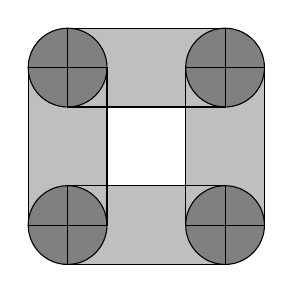
\begin{tikzpicture}
    \fill[lightgray] (0.5,0) rectangle (2.5,1);
    \fill[lightgray] (0.5,2) rectangle (2.5,3);
    \fill[lightgray] (0,0.5) rectangle (1,2.5);
    \fill[lightgray] (2,0.5) rectangle (3,2.5);
    \filldraw[fill=gray,draw=black](0.5,0.5) circle (0.5);
    \filldraw[fill=gray,draw=black](2.5,0.5) circle (0.5);
    \filldraw[fill=gray,draw=black](0.5,2.5) circle (0.5);
    \filldraw[fill=gray,draw=black](2.5,2.5) circle (0.5);
    \draw[black] (0.5,0) rectangle (2.5,1);
    \draw[black] (0.5,2) rectangle (2.5,3);
    \draw[black] (0,0.5) rectangle (1,2.5);
    \draw[black] (2,0.5) rectangle (3,2.5);
    \end{tikzpicture}}\quad
  \subfloat[]{\label{fig:atc:gps}
    \begin{forest}
      [\name{AosXMonotoneTraits\_2},for tree={concept,edge={-latex}}
        % forked edges
        [\name{AosDirectionalXMonotoneTraits\_2}
          [\name{GeneralPolygonSetTraits\_2}]
        ]
      ]
    \end{forest}}
  \caption[]{%
    \subref{fig:csp}~A general polygon with holes bounded by circular arcs and line segments.
    \subref{fig:atc:gps}~The general point-set cluster.}
  \label{fig:bso2}
\end{figure}

An arrangement data structure is internally used to represent the
point set maintained by the general polygon-set; it is possible to
obtain it and apply further operations on it, as demonstrated by the
code excerpt in Listing~\ref{lst:py:circleSegmentPolygonsArr}.

\begin{lstfloat}
\lstinputlisting[style=pythonFramedStyle,%
                 basicstyle=\normalsize,%
                 firstline=64,%
                 label={lst:py:circleSegmentPolygonsArr},%
                 caption={Extracting the arrangement from a point set.}]%
                 {../../../src/python_scripts/cgalpy_examples/circle_segment_polygons.py}
\end{lstfloat}

The bindings for the \iiDArrangementsPackage{} package includes
bindings for the geometry traits and the DCEL suitable for Boolean
operations. In particular, the traits must model the concept
\cppLstinline{GeneralPolygonSetTraits\_2}; see
Figure~\ref{fig:atc:gps}.

% -----------------------------------------------------------------------------
\subsection{2D Minkowski Sums}
\label{ssec:modules:ms2}
% -----------------------------------------------------------------------------
Given two sets of points $\calA, \calB \in \Rd$ their Minkowski sum,
denoted by $\calA \oplus \calB$, is their point-wise sum, namely the
set $\{a+b |\, a \in \calA,b \in \calB\}$. The \cgal{} package
\iiDMinkowskiSumsPackage{} contains functions that compute the planar
Minkowski sums of two polygons and the planar Minkowski sum of a
simple polygon and a disc---an operation also referred to as
offsetting or dilating a polygon. The package also supports inner
offsetting a polygon (also referred to as insetting), which is
equivalent to the complement of the offset of a disk and the
complement of a polygon~\cite{cgal:w-rms2-21a}. The
\iiDMinkowskiSumsPackage{} module is not associated with any \cmake{}
flags (besides the flag \cmakeLstinline{MINKOWSKI_SUM_2_BINDINGS},
which indicates whether to generate bindings for this module). As with
the \iiDRegularizedBooleanSetOperationsPackage{} package, the
operations supported by this package depends on the
\iiDandiiiDGeometryKernelPackage{}, \iiDArrangementsPackage{}, and
\iiDPolygonsPackage{} packages. Generating bindings for the
\iiDMinkowskiSumsPackage{} module does not require thought enabling
the bindings for the \iiDArrangementsPackage{} module (similar to the
case of generating bindings of Boolean operations on (linear) polygons
supported by the \iiDRegularizedBooleanSetOperationsPackage{}
package). The result of the inset and offset operations is a general
polygon bounded by line segments and circular arc. Thus, binding for
such a type is generated as well.

The function instance \cppLstinline{CGAL::minkowski_sum()} is
extremely overloaded. It can be used to compute the Minkowski sum of
two polygons either applying the \emph{convex-decomposition} approach
or the \emph{reduced-convolution} approach. When applying the
\emph{convex-decomposition} approach we first decompose each summand
into convex sub-polygons. The function template
\cppLstinline{CGAL::minkowski\_sum_by_full_convolution_2()} applies a
third approach, namely \emph{full convolution}. For more information
on the various approaches refer to the manual.

There are two overloaded function templates
\cppLstinline{CGAL::minkowski_sum()} that apply the
\emph{reduced-convolution} approach; both accepts the two polygons as
input; one also accepts a specific geometry traits as input (while the
other constructs and uses a default one). Each type of the summands
must represent either a simple polygon or a polygon with holes. The
signature of the former is shown in Listing~\ref{lst:cpp:minkSum},
where \cppLstinline{PolygonType1} and \cppLstinline{PolygonType2} can
be substituted either with \cppLstinline{Polygon_2} or with
\cppLstinline{Polygon_with_holes_2}.
%
Thus, given a specific kernel and container types, we get eight
overloaded instances that apply the \emph{reduced-convolution}
approach in total. (The Container type determines the representation
of the polygon extreme points in memory.)

\begin{lstfloat}
  \begin{lstlisting}[style=cppFramedStyle,basicstyle=\normalsize,
                     label={lst:cpp:minkSum},
                     caption={The signature of one of the \cppLstinline{CGAL::minkowski_sum_2} overloaded function templates.}]
template <typename Kernel, typename Container>
Polygon_with_holes_2<Kernel, Container>
minkowski_sum_2(const PolygonType1<Kernel, Container>& p,
                const PolygonType2<Kernel, Container>& q)
\end{lstlisting}
\end{lstfloat}

There are two sets of function templates
\cppLstinline{CGAL::minkowski_sum()} that apply the
\emph{convex-decomposition} approach; all functions accepts the two
polygons as input; functions in one set also accept a specific
geometry traits as input. As with the functions that apply the
\emph{reduced-convolution} approach, each type of the summands must be
substituted either with a type that represents a simple polygon or a
type that represents a polygon with holes. Each set consists of two
function templates; one is parameterized with the type that represents
a single decomposition strategy that should be applied to both
summands and another one that is parameterized with two types that
represents two decomposition strategies that should be applied to the
two summands, respectively. The package provides four types of
decomposition strategies; however, only two can be applies to polygon
width holes. Bellow are the signatures of the two functions that do
not accept a traits parameter.

We get 10~overloaded instances of functions that apply the
\emph{convex-decomposition} approach, do not accept a traits
parameter, and are parameterized with a single decomposition
strategy. We get 36~overloaded instances of functions that apply the
\emph{convex-decomposition} approach, do not accept a traits
parameter, and are parameterized with two decomposition
strategies. Thus, given a specific kernel and container types, we get
$2 \times (10 + 36) = 92$ overloaded instances of functions that apply
the \emph{convex-decomposition} approach.

The \cppLstinline{approximated_inset_2(P, r, eps, oi)} function
template accepts a polygon $P$, an inset radius $r$, (a floating-point
number\index{number!floating-point}) $\epsilon > 0$, and an output
iterator\index{iterator!output} \cppLstinline{oi}, whose value-type
must be an instance of the class template
\cppLstinline{Gps_circle_segment_traits_2::Polygon_2}. It constructs
an approximation of the inset of $P$ by the radius $r$, where the
approximation error is bounded by $\epsilon$. The function returns the
polygons that approximate the inset polygon through the output
iterator \cppLstinline{oi}.

The code excerpt in Listing~\ref{lst:py:approxInset} demonstrates the
construction of an approximated inner offset; see
Figure~\ref{fig:ms2:inset}.

\begin{lstfloat}
\lstinputlisting[style=pythonFramedStyle,%
                 basicstyle=\normalsize,%
                 firstline=35,%
                 label={lst:py:approxInset},%
                 caption={Computing the approximated inner offset.}]%
                 {../../../src/python_scripts/cgalpy_examples/approx_inset.py}
\end{lstfloat}

\begin{SCfigure}[][!htp]
 \begin{tikzpicture}[scale=0.4]
    \coordinate (c1) at (8,3);
    \coordinate (p11) at (8.94868,3.31623);
    \coordinate (p12) at (7.05132,3.31623);
    %
    \coordinate (c2) at (6,7);
    \coordinate (p21) at (6.78087,6.3753);
    \coordinate (p22) at (7,7);      %\draw (6,9) circle (3pt);


    \filldraw [color=polyADarkColor,fill=polyALightColor,thick]
      (4, 0)--(7,0)--(8,3)--(9,0)--(13,0)--(13,8)--(7,8)--(7,9)--
      (13,9)--(13,14)--(0,14)--(0,12)--(6,9)--(6,7)--(2,2)--cycle;
    \filldraw [color=polyCDarkColor,fill=polyCLightColor,thick]
      let \p1 = ($(p11) - (c1)$),
        \p2 = ($(p12) - (c1)$),
        \n0 = {veclen(\x1,\y1)}, % radius
        \n1 = {atan2(\y1,\x1)},  % initial angle
        \n2 = {atan2(\y2,\x2)},  % Final angle
        \p3 = ($(p21) - (c2)$),
        \p4 = ($(p22) - (c2)$),
        \n3 = {veclen(\x3,\y4)}, % radius
        \n4 = {atan2(\y3,\x4)},  % initial angle
        \n5 = {atan2(\y3,\x4)}   % Final angle
      in
        (7,7)--(12,7)--(12,1)--(9.72076,1)--(9.29057,2.29057)--(p11)arc(\n1:\n2:\n0)--
        (6.3932,1.34189)--(6.27924,1)--(4.41421,1)--(3.34,2.07422)--(3.53148,2.31357)--
        (p21)arc(\n4:\n5:\n3)--cycle;
    \filldraw [color=polyCDarkColor,fill=polyCLightColor,thick]
      (1,13)--(12,13)--(12,10)--(7,10)--
      (6.5,9.86603)--
      (6.44721,9.89443)--(4.78885,10.7236)--(1,12.618)--(1,13)--cycle;
      %\draw (7,9) circle (3pt);
      %\draw (6,9) circle (3pt);
  \end{tikzpicture}
  \caption{%
    The inset (yellow) of a polygon (blue) with a tight corridor
    consists of two general polygons bounded by line segments and
    circular arcs.}
  \label{fig:ms2:inset}
\end{SCfigure}

% -----------------------------------------------------------------------------
\subsection{2D Triangulation Bindings}
\label{ssec:modules:tri2}
% -----------------------------------------------------------------------------
A triangulation of a set of points $\calP$ in \Rtwo is a partition of
the convex hull of $\calP$ into triangles whose vertices are the
points of $\calP$. Together with the unbounded face having the convex
hull boundary as its frontier, the triangulation forms a partition of
\Rtwo. Any two facets (2-face) are either disjoint or share a common
edge (1-face) or vertex (0-face). A triangulation can be described as
a simplicial complex. The binding module
\iiDTriangulationsPackage{} consists of bindings of types provided by
the \cgal{} packages \iiDTriangulationsPackage{} and
\iiDPeriodicTriangulationsPackage{}. Table~\ref{tab:tri2} lists the
\cmake{} flags associated with the \iiDTriangulationsPackage{}
module.

%%%%%%%% 2D Triangulation Module Flags
\begin{table}[!htp]
  \caption{\iiDTriangulationsPackage{} module flags.}
  \centering\begin{tikzpicture}
  \matrix (first) [tableModuleFlags,
    column 1/.style={nodes={text width=16.0em}},
    column 3/.style={nodes={text width=5.7em}},
    column 4/.style={nodes={text width=21.6em}},
    row 6/.append style={nodes={minimum height=2.8em}}
  ] {
    Name & Type & Default & Description\\
    \cmakeLstinline{TRI2\_NAME} & String & \myLstinline{plain} &
      The 2D triangulation type\\
    \cmakeLstinline{TRI2\_VERTEX\_WITH\_INFO}      & Boolean & \myLstinline{false} & Determines whether the vertex type is extented\\
    \cmakeLstinline{TRI2\_FACE\_WITH\_INFO}        & Boolean & \myLstinline{false} & Determines whether the face type is extented\\
    \cmakeLstinline{TRI2\_INTERSECTION\_TAG\_NAME} & String  & \myLstinline{ncirc} & The intersection tag\\
    \cmakeLstinline{TRI2\_HIERARCHY}               & Boolean & \myLstinline{false} & Determines whether to generate the binding for a hierarchy triangulation\\
  };
  \end{tikzpicture}
  \label{tab:tri2}
\end{table}

The \iiDTriangulationsPackage{} package~\cite{cgal:y-t2-21a}
provides several class templates, instances of which can be used to
represent a variety of 2D triangulations. In particular, the package
provides the following class templates:
\begin{compactenum}
\item \cppLstinline{Triangulation\_2<Traits, Tds>},
\item \cppLstinline{Regular\_triangulation\_2<Traits, Tds>},
\item \cppLstinline{Delaunay\_triangulation\_2<Traits, Tds>},
\item \cppLstinline{Constrained\_triangulation\_2<Traits, Tds, Itag>},
\item \cppLstinline{Constrained\_Delaunay\_triangulation\_2<Traits, Tds, Itag>}, and
\item \cppLstinline{Triangulation\_hierarchy\_2<Triangulation\_2>}
\end{compactenum}
Instance of the \cppLstinline{Delaunay\_triangulation\_2<>} and
\cppLstinline{Regular\_triangulation\_2<>} class templates can be used
to represent Delaunay and regular triangulation, respectively. In a
regular triangulation points have an associated weight, and some
points can be hidden and do not result in vertices in the
triangulation. The class template
\cppLstinline{Triangulation\_hierarchy\_2} enables fast point location
queries. When instantiated its template parameter must be substituted
with an instance of any other triangulation class template.

The \iiDPeriodicTriangulationsPackage{}
package~\cite{cgal:k-pt2-13-21a} supports triangulations of sets of
points in the two-dimensional flat torus~\cite{ct-cpt-09}. This
package provides the class templates
\begin{compactenum}
\item \cppLstinline{Periodic\_2\_triangulation\_2<Traits, Tds>},
\item \cppLstinline{Periodic\_2\_Delaunay\_triangulation\_2<Traits, Tds>}
\item \cppLstinline{Periodic\_2\_triangulation\_hierarchy\_2<PeriodicTriangulation>}
\end{compactenum}

The \cmake{} flag \cmakeLstinline{TRI2\_NAME} specifies the particular
type of triangulation, bindings for which should be generated; see
Table~\ref{tab:tri2:names}.

\begin{table}[!htp]
  \caption{2D triangulation name options}
  \centering\begin{tikzpicture}
  \matrix (first) [tableName,
    column 1/.style={nodes={text width=11.5em}},
    column 2/.style={nodes={text width=37.5em}}
  ] {
    \cmakeLstinline{TRI2\_NAME} & Type\\
    \myLstinline{plain} & \cppLstinline{Triangulation\_2<Traits, Tds>}\\
    \myLstinline{regular} & \cppLstinline{Regular\_triangulation\_2<Traits, Tds>}\\
    \myLstinline{delaunay} & \cppLstinline{Delaunay\_triangulation\_2<Traits, Tds>}\\
    \myLstinline{constrained} & \cppLstinline{Constrained\_triangulation\_2<Traits, Tds, Itag>}\\
    \myLstinline{constrainedDelaunay} & \cppLstinline{Constrained\_Delaunay\_triangulation\_2<Traits, Tds, Itag>}\\
    \myLstinline{periodicPlain} & \cppLstinline{Periodic\_2\_triangulation\_2<Traits, Tds>}\\
    \myLstinline{periodicDelaunay} & \cppLstinline{Periodic\_2\_Delaunay\_triangulation\_2<Traits, Tds>}\\
  };
  \end{tikzpicture}
  \label{tab:tri2:names}
\end{table}

%% \cppLstinline{TriangulationTraits\_2}
%% \cppLstinline{RegularTriangulationTraits\_2}
%% \cppLstinline{DelaunayTriangulationTraits\_2}
%% \cppLstinline{ConstrainedTriangulationTraits\_2}
%% \cppLstinline{ConstrainedDelaunayTriangulationTraits_2}
%% \cppLstinline{AlphaShapeTraits\_2}
%% \cppLstinline{WeightedAlphaShapeTraits\_2}
%% \cppLstinline{Periodic\_2TriangulationTraits\_2}
%% \cppLstinline{Periodic\_2DelaunayTriangulationTraits\_2}
%% \cppLstinline{Periodic\_3AlphaShapeTraits\_2}
When any template above is instantiated the template parameter
\cppLstinline{Traits} must be substituted with a model of a suitable
geometric traits concept; this model is referred to as the geometric
traits class; it provides the type of points to use as well as
elementary operations on them. The type of traits used for the
generated bindings is determined based on the selection of the
triangulation type as explained below. It is conveniently defined in
C++ as \cppLstinline{Dt::Geom\_traits}, where \cppLstinline{Dt} is a
triangulation instance. This type is exposed as a Python attribute
with the same name under \pyLstinline{Triangulation\_2} (which in turn
is nested under the Python namespace \pyLstinline{Tri2}).
Figure~\ref{tab:tri2:concept-hierarchy} depicts the 2D triangulation
traits concept hierarchy. Any kernel instance is a model of any
non-periodic traits concept; thus, when one of the templates
\begin{compactenum}
\item \cppLstinline{Triangulation\_2<Traits, Tds>},
\item \cppLstinline{Regular\_triangulation\_2<Traits, Tds>},
\item \cppLstinline{Delaunay\_triangulation\_2<Traits, Tds>},
\item \cppLstinline{Constrained\_triangulation\_2<Traits, Tds, Itag>}, or
\item \cppLstinline{Constrained\_Delaunay\_triangulation\_2<Traits, Tds, Itag>}
\end{compactenum}
is instantiated, the \cppLstinline{Traits} parameter is substituted
with the \cppLstinline{Kernel} type (the selected kernel; see
Section~\ref{ssec:modules:kernel}). When one of the templates
\begin{compactenum}
\item \cppLstinline{Periodic\_2\_triangulation\_2<Traits, Tds>} or
\item \cppLstinline{Periodic\_2\_Delaunay\_triangulation\_2<Traits, Tds>}
\end{compactenum}
is instantiated, the \cppLstinline{Traits} parameter is substituted
with \cppLstinline{Periodic\_2\_triangulation\_traits\_2<Kernel>} or
\cppLstinline{Periodic\_2\_Delaunay\_triangulation\_traits_2<Kernel>},
respectively.
%
Observe that when a Delaunay triangulation instance is used to define
an alpha shape type (see Section~\ref{ssec:modules:as2}), the traits
parameter must be substituted with a traits class that models the
\cppLstinline{AlphaShapeTraits\_2} concept. Similarly, when a regular
triangulation instance is used to define an fixed alpha shape type
(see Section~\ref{ssec:modules:as2}, the traits parameter must be
substituted with a traits class that models the
\cppLstinline{WeightedAlphaShapeTraits\_2} concept. Also in these
cases the selected kernel serves as the traits.

\begin{figure}[!htp]
  \def\name#1{\scriptsize\cppLstinline{#1}}
  \tikzset{%
    concept/.style={rectangle,rounded corners,align=center,
      draw,fill=white,blur shadow,% drop shadow%
    }
  }
  \forestset{
    my tree style/.style={
      for tree={concept,
        parent anchor=south,
        child anchor=north,
        edge={->,>=stealth,black,thick},
        edge path={% |-| style branches from parent to child
          \noexpand\path [draw, \forestoption{edge}] (!u.parent anchor)--(.child anchor)\forestoption{edge label};
        },
        if n children=3{% if a node has 3 children
          for children={% align the middle child with its parent
            if n=2{calign with current}{}
          }
        }{},
      }
    }
  }
  \centering%
  \begin{forest}
    my tree style
    [ \name{TriTr2}
      [ \name{RegularTriTr2}
        [ \name{WeightedAlphaShapeTr2} ]
      ]
      [ \name{Pr2TriTr2},name=p ]
      [ \name{DelaunayTriTr2},name=d
        [ \name{Pr2DelaunayTriTr2},name=pd
	  [ \name{Pr2AlphaShapeTr2} ]
        ]
        [ \name{AlphaShapeTr2} ]
      ]
      [ \name{ConstrainedTriTr2}
        [ \name{ConstrainedDelaunayTriTr2},name=cd ]
      ]
    ]
    \draw[->,>=stealth] (d.parent anchor)--(cd.child anchor);
    \draw[->,>=stealth] (p.parent anchor)--(pd.child anchor);
  \end{forest}
  \caption{The 2D triangulation traits concept hierarchy.
    \cppLstinline{Triangulation}, \cppLstinline{Periodic\_2} and
    \cppLstinline{Traits\_2} are abbreviated as \cppLstinline{Tri},
    \cppLstinline{Pr2}, and \cppLstinline{Tr2},
    respectively.}
  \label{tab:tri2:concept-hierarchy}
\end{figure}

The type that substitutes the \cppLstinline{Tds}
parameter models the concept
\cppLstinline{TriangulationDataStructure\_2}. An object of this type
stores the combinatorial structure of the triangulation; it is an
instance of the class template
\cppLstinline{Triangulation\_data\_structure\_2<VertexBase, FaceBase>}.

The types that substitute the \cppLstinline{VertexBase} and
\cppLstinline{FaceBase} template parameters when the template
\cppLstinline{Triangulation\_data\_structure\_2<VertexBase, FaceBase>}
is instantiated represent the type of the vertex and the type of the
face of the triangulation, respectively; they must model the concepts
\cppLstinline{TriangulationDSVertexBase\_2} and
\cppLstinline{TriangulationDSFaceBase\_2}, respectively. If the
binding is generated for a periodic triangulation, these parameters
must be substituted with types that also model the concepts
\cppLstinline{Periodic\_2TriangulationDSVertexBase\_2} and
\cppLstinline{Periodic\_2TriangulationDSFaceBase\_2}, respectively.
If the triangulation is used to define an alpha shape type, these
parameters must be substituted with types that also model the concepts
\cppLstinline{AlphaShapeVertex\_2} and
\cppLstinline{AlphaShapeFace\_2}, respectively; see
Section~\ref{ssec:modules:as2}. Finally, if the binding is generated
for a hierarchy triangulation, e.g., an instance of the template
parameter
\cppLstinline{Triangulation\_hierarchy\_2<Triangulation\_2>}, the
\cppLstinline{VertexBase} template parameter must be substituted with
a model of the concept
\cppLstinline{TriangulationHierarchyVertexBase\_2}. (Observe that
there is no special requirements on the type that substitutes the
\cppLstinline{FaceBase} parameter in this case.) The final vertex
type is selected accordingly as follows.

%% 2D Triangulation Vertex Selection
The type \cppLstinline{Vb} is defined as the vertex base type.  If
bindings is generated for a periodic triangulation, the type
\cppLstinline{Vb} is defined as
\cppLstinline{Periodic\_2\_triangulation\_vertex\_base\_2<Traits>};
otherwise, if bindings is generated for an instance of
\cppLstinline{Regular\_triangulation\_vertex\_base\_2<Kernel>}, the
type \cppLstinline{Vb} is defined as
\cppLstinline{Regular\_triangulation\_vertex\_base\_2<Traits>};
otherwise, the type \cppLstinline{Vb} is defined as
\cppLstinline{Triangulation\_vertex\_base\_2<Traits>}.
%
If the \cmake{} flag \cmakeLstinline{TRI2\_VERTEX\_WITH\_INFO} is set
to \myLstinline{true}, the type \cppLstinline{Vbi} is defined as
\cppLstinline{Triangulation\_vertex\_base\_with\_info\_2<Data, Kernel,
  Vb>}, where \cppLstinline{Data} is defined as the generic Python
object \cppLstinline{bp::object}; see Section~\ref{sec:code:ae};
otherwise the type \cppLstinline{Vbi} is defined as \cppLstinline{Vb}.
%
If the \cmake{} flag \cmakeLstinline{TRI2\_HIERARCHY} is set
to \myLstinline{true}, the type \cppLstinline{Vbih} is defined as
\cppLstinline{Triangulation\_hierarchy\_vertex\_base\_2<Vbi>}; otherwise
the type \cppLstinline{Vbih} is defined as \cppLstinline{Vbi}.
%
Finally, if the triangulation is used to define an alpha shape type,
the final type \cppLstinline{V} (that substitutes the
\cppLstinline{VertexBase} parameter) is defined as
\cppLstinline{Alpha\_shape\_vertex\_base\_2<Traits, Vbih,
  ExactComparison>}, where \cppLstinline{ExactComparison} is
substituted with either \cppLstinline{true} or \cppLstinline{false}
based on the setting of the \cmake{} flag
\cmakeLstinline{AS2\_EXACT\_COMPARISON}; see
Table~\ref{tab:as2}. Otherwise, \cppLstinline{V} is defined as
\cppLstinline{Vbih}.
%
The final vertex type is conveniently defined in C++ as
\cppLstinline{Dt::Vertex}, where \cppLstinline{Dt} is the
triangulation instance. This type is exposed as a Python attribute
with the same name under \pyLstinline{Triangulation_2}.

The final face type is determined in a similar fashion. The only
difference between the selections of the vertex and face types is that
the setting of the \cmake{} flag \cmakeLstinline{TRI2\_HIERARCHY} does
not have an effect on the face type selection. The final face type is
conveniently defined in C++ as \cppLstinline{Dt::Face}, where
\cppLstinline{Dt} is the triangulation instance. This type is also
exposed as a Python attribute with the same name under
\pyLstinline{Triangulation_2}.

The \cmake{} Boolean flag \cmakeLstinline{TRI2\_HIERARCHY} indicates
whether the type of triangulation, bindings for which should be
generated, is an instance of one of the triangulation hierarchy
templates, namely,
\cppLstinline{Triangulation\_hierarchy\_2<Triangulation\_2>} and
\cppLstinline{Periodic_triangulation\_hierarchy\_2<PeriodicTriangulation\_2>}.
The template parameter in both cases is substituted with the
triangulation selected via the \cmake{} flag
\cmakeLstinline{TRI2\_NAME}, which also determines whether to use the
non-periodic or periodic version above.

% -----------------------------------------------------------------------------
\subsection{2D Alpha Shape Bindings}
\label{ssec:modules:as2}
% -----------------------------------------------------------------------------
The alpha shape (a.k.a.\ alpha complex) of a set of points is one of
several notions of a shape formed by the set. Given a set of points
sampled in a 2D body, an alpha shape is demarcated by a frontier,
which is a linear approximation of the original boundary of the
body. A two-dimensional alpha shape object maintains an underlying
triangulation of a set of input points in the plane. There are two
distinguished versions of alpha shapes as follows. Basic alpha shapes
are based on the Delaunay triangulation and weighted alpha shapes are
based on its generalization, the regular triangulation, where the
euclidean distance is replaced by the power to weighted points.  The
package \iiDAlphaShapesPackage{}~\cite{cgal:d-as2-21a} provides the
class template \cppLstinline{Alpha\_shape\_2<Dt,
  ExactAlphaComparisonTag>}. In a 2D alpha shape object represented by
an instance of this class template each $k$-simplex of the underlying
triangulation is associated with an interval that specifies for which
values of $\alpha$ the $k$-simplex belongs to the alpha shape.
Table~\ref{tab:as2} lists the \cmake{} flags associated with the
\iiDAlphaShapesPackage{} module.

%%%%%%%% 2D Alpha Shape Module flags
\begin{table}[!htp]
  \caption{\iiiDAlphaShapesPackage{} module flags}
  \centering\begin{tikzpicture}
  \matrix (first) [tableModuleFlags,
    column 1/.style={nodes={text width=16em}},
    column 3/.style={nodes={text width=5.7em}},
    column 4/.style={nodes={text width=21.6em}}
  ] {
    Name & Type &  Default & Description\\
    \myLstinline{AS2\_EXACT\_COMPARISON} & Boolean & \myLstinline{false} &
      Determines whether to apply exact comparisons\\
  };
 \end{tikzpicture}
 \label{tab:as2}
\end{table}

% -----------------------------------------------------------------------------
\subsection{3D Triangulation Bindings}
\label{ssec:modules:tri3}
% -----------------------------------------------------------------------------
A triangulation of a set of points $\calP$ in \Rthree is a partition
of the convex hull of $\calP$ into tetrahedra whose vertices are the
points of $\calP$. Similar to the two-dimensional triangulation,
together with the unbounded cell having the convex hull boundary as
its frontier, the triangulation forms a partition of \Rthree. Any two
cells (3-face) are either disjoint or share a common facet (2-face),
edge (1-face) or vertex (0-face).  The binding module
\iiiDTriangulationsPackage{} consists of bindings of types provided by
the \cgal{} packages \iiiDTriangulationsPackage{} and
\iiiDPeriodicTriangulationsPackage{}. Table~\ref{tab:tri3} lists the
\cmake{} flags associated with the \iiiDTriangulationsPackage{}
module.

%%%%%%%% 3D Triangulation Module Flags
\begin{table}[!htp]
  \caption{\iiiDTriangulationsPackage{} module flags. For the default
  value of the traits name see Table~\ref{tab:tri3:traits-default}.}
  \centering\begin{tikzpicture}
  \matrix (first) [tableModuleFlags] {
    Name & Type & Default & Description\\
    \cmakeLstinline{TRI3\_NAME}                   & String & \myLstinline{plain}    & The 3D triangulation type\\
    \cmakeLstinline{TRI3\_CONCURRENCY\_NAME}      & String & \myLstinline{sequential} & The concurrency method\\
    \cmakeLstinline{TRI3\_LOCATION\_POLICY\_NAME} & String & \myLstinline{compact}    & The location policy\\
  };
  \end{tikzpicture}
  \label{tab:tri3}
\end{table}

The \iiiDTriangulationsPackage{} package~\cite{cgal:pt-t3-21a}
provides several class templates, instances of which can be used to
represent a variety 3D triangulations. In particular, the package
provides the following class templates:
\begin{compactenum}
\item \cppLstinline{Triangulation\_3<Traits, Tds, Slds>},
\item \cppLstinline{Regular\_triangulation\_3<Traits, Tds, Slds>}, and
\item \cppLstinline{Delaunay\_triangulation\_3<Traits, Tds, LocationPolicy, Slds>}
\item \cppLstinline{Triangulation\_hierarchy\_3<Triangulation\_3>}
\end{compactenum}
Instance of the \cppLstinline{Delaunay\_triangulation\_3<>} and
\cppLstinline{Regular\_triangulation\_3<>} class templates can be used
to represent Delaunay and regular triangulation, respectively. In a
regular triangulation points have an associated weight, and some
points can be hidden and do not result in vertices in the
triangulation. When instantiated its template parameter must be
substituted with an instance of any other triangulation class
template.

The \iiiDPeriodicTriangulationsPackage{}
package~\cite{cgal:ct-pt3-21a} supports triangulations of sets of
points in the three-dimensional flat torus~\cite{ct-cpt-09}. This
package provides the class templates
\begin{compactenum}
\item \cppLstinline{Periodic\_3\_triangulation\_3<Traits, Tds>},
\item \cppLstinline{Periodic\_3\_regular\_triangulation\_3<Traits, Tds>}, and
\item \cppLstinline{Periodic\_3\_Delaunay\_triangulation\_3<Traits, Tds>}
\item \cppLstinline{Periodic\_3\_triangulation\_hierarchy\_3<PeriodicTriangulation>}
\end{compactenum}

The \cmake{} flag \myLstinline{TRI3\_NAME} specifies the particular
types of triangulations, bindings for which should be generated; see
Table~\ref{tab:tri3:names}.

\begin{table}[!htp]
  \caption{3D triangulation name options}
  \centering\begin{tikzpicture}
  \matrix (first) [tableName,
    column 1/.style={nodes={text width=10em}},
    column 2/.style={nodes={text width=39em}}
  ] {
    \myLstinline{TRI3\_NAME} & Type\\
    \myLstinline{plain} & \cppLstinline{Triangulation\_3<Traits, Tds, Slds>}\\
    \myLstinline{regular} & \cppLstinline{Regular\_triangulation\_3<Traits, Tds, Slds>}\\
    \myLstinline{delaunay} & \cppLstinline{Delaunay\_triangulation\_3<Traits, Tds, LocationPolicy, Slds>}\\
    \myLstinline{periodicPlain} & \cppLstinline{Periodic\_3\_triangulation\_3<Traits, Tds>}\\
    \myLstinline{periodicRegular} & \cppLstinline{Periodic\_3\_regular\_triangulation\_3<Traits, Tds>}\\
    \myLstinline{periodicDelaunay} & \cppLstinline{Periodic\_3\_Delaunay\_triangulation\_3<Traits, Tds>}\\
  };
  \end{tikzpicture}
  \label{tab:tri3:names}
\end{table}

%% \cppLstinline{TriangulationTraits\_3}
%% \cppLstinline{RegularTriangulationTraits\_3}
%% \cppLstinline{DelaunayTriangulationTraits\_3}
%% \cppLstinline{AlphaShapeTraits\_3}
%% \cppLstinline{FixedAlphaShapeTraits\_3}
%% \cppLstinline{WeightedAlphaShapeTraits\_3}
%% \cppLstinline{FixedWeightedAlphaShapeTraits\_3}
%% \cppLstinline{Periodic\_3TriangulationTraits\_3}
%% \cppLstinline{Periodic\_3RegularTriangulationTraits\_3}
%% \cppLstinline{Periodic\_3DelaunayTriangulationTraits\_3}
%% \cppLstinline{Periodic\_3AlphaShapeTraits\_3}
When any template above is instantiated the template parameter
\cppLstinline{Traits} must be substituted with a model of a suitable
geometric traits concept; this model is referred to as the geometric
traits class; it provides the type of points to use as well as
elementary operations on them. The type of traits used for the
generated bindings is determined based on the selection of the
triangulation type as explained below. It is conveniently defined in
C++ as \cppLstinline{Dt::Geom\_traits}, where \cppLstinline{Dt} is the
triangulation instance. This type is exposed as a Python attribute
with the same name under \pyLstinline{Triangulation\_3} (which in turn
is nested under the Python namespace \pyLstinline{Tri3}).
Figure~\ref{tab:tri3:concept-hierarchy} depicts the 2D triangulation
traits concept hierarchy. Any kernel instance is a model of any
non-periodic traits concept; thus, when one of the templates
\begin{compactenum}
\item \cppLstinline{Triangulation\_3<Traits, Tds>},
\item \cppLstinline{Regular\_triangulation\_3<Traits, Tds>}, abd
\item \cppLstinline{Delaunay\_triangulation\_3<Traits, Tds>}
\end{compactenum}
is instantiated, the \cppLstinline{Traits} parameter is substituted
with the \cppLstinline{Kernel} type (the selected kernel; see
Section~\ref{ssec:modules:kernel}). When one of the templates
\begin{compactenum}
\item \cppLstinline{Periodic\_3\_triangulation\_3<Traits, Tds>},
\item \cppLstinline{Periodic\_3\_regular\_triangulation\_3<Traits, Tds>}, or
\item \cppLstinline{Periodic\_3\_Delaunay\_triangulation\_3<Traits, Tds>}
\end{compactenum}
is instantiated, the \cppLstinline{Traits} parameter is substituted
with \cppLstinline{Periodic\_3\_triangulation\_traits\_3<Kernel>},
\cppLstinline{Periodic\_3\_regular\_triangulation\_traits_3<Kernel>}, or
\cppLstinline{Periodic\_3\_Delaunay\_triangulation\_traits_3<Kernel>},
respectively.
%
Observe that when a Delaunay triangulation instance is used to define
either a plain or a fixed alpha shape type (see
Section~\ref{ssec:modules:as3}), the traits parameter must be
substituted with a traits class that models either the
\cppLstinline{AlphaShapeTraits\_3} or the
\cppLstinline{FixedAlphaShapeTraits\_3} concept,
respectively. Similarly, when a regular triangulation instance is used
to define either a plain or a fixed alpha shape type (see
Section~\ref{ssec:modules:as3}, the traits parameter must be
substituted with a traits class that models either the
\cppLstinline{WeightedAlphaShapeTraits\_3} or the
\cppLstinline{FixedWeightedAlphaShapeTraits\_3} concept,
respectively. Also in these cases the selected kernel serves as the
traits.

\begin{figure}[!htp]
  \def\name#1{\scriptsize\cppLstinline{#1}}
  \tikzset{%
    concept/.style={rectangle,rounded corners,align=center,
      draw,fill=white,blur shadow,% drop shadow%
    }
  }
  \forestset{
    my tree style/.style={
      for tree={concept,
        parent anchor=south,
        child anchor=north,
        edge={->,>=stealth,black,thick},
        edge path={% |-| style branches from parent to child
          \noexpand\path [draw, \forestoption{edge}] (!u.parent anchor)--(.child anchor)\forestoption{edge label};
        },
        if n children=3{% if a node has 3 children
          for children={% align the middle child with its parent
            if n=2{calign with current}{}
          }
        }{},
      }
    }
  }
  \centering
  \begin{forest}
    my tree style
    [ \name{TriTr3}
      [ \name{RegularTriTr3},name=r
        [ \name{WeightedASTr3} ]
        [ \name{FixedWeightedASTr3} ]
      ]
      [ \name{Periodic\_3TriTr3},name=p
        [ \name{Pr3RegularTriTr3},name=pr ]
      ]
      [ \name{DelaunayTriTr3},name=d
        [ \name{Pr3DelaunayTriTr3},name=pd
	  [ \name{Pr3ASTr3} ]
        ]
        [ \name{ASTr3} ]
        [ \name{FixedASTr3} ]
      ]
    ]
    \draw[->,>=stealth] (r.parent anchor)--(pr.child anchor);
    \draw[->,>=stealth] (p.parent anchor)--(pd.child anchor);
  \end{forest}
  \caption{The 3D triangulation traits concept hierarchy.
    \cppLstinline{Triangulation}, \cppLstinline{AlphaShape},
    \cppLstinline{Traits\_3} and \cppLstinline{Periodic\_3} are
    abbreviated as \cppLstinline{Tri}, \cppLstinline{AS},
    \cppLstinline{Pr3}, and \cppLstinline{Tr3}, respectively.}
  \label{tab:tri3:concept-hierarchy}
\end{figure}

The type that substitutes the \cppLstinline{Tds}
parameter models the concept
\cppLstinline{TriangulationDataStructure\_3}. An object of this type
stores the combinatorial structure of the triangulation; it is an
instance of the class template
\cppLstinline{Triangulation\_data\_structure\_3<VertexBase, CellBase,
  ConcurrencyTag>}.

The types that substitute the \cppLstinline{VertexBase} and
\cppLstinline{CellBase} template parameters when the template
\cppLstinline{Triangulation\_data\_structure\_3<VertexBase, CellBase>}
is instantiated represent the type of the vertex and the type of the
cell of the triangulation, respectively; they must model the concepts
\cppLstinline{TriangulationDSVertexBase\_3} and
\cppLstinline{TriangulationDSCellBase\_3}, respectively. If the
binding is generated for a periodic triangulation, these parameters
must be substituted with types that also model the concepts
\cppLstinline{Periodic\_3TriangulationDSVertexBase\_3} and
\cppLstinline{Periodic\_3TriangulationDSCellBase\_3}, respectively.
If the triangulation is used to define a plain alpha shape type, these
parameters must be substituted with types that model the concepts
\cppLstinline{AlphaShapeVertex\_3} and
\cppLstinline{AlphaShapeCell\_3}, respectively; see
Section~\ref{ssec:modules:as3}. If the triangulation is used to define
a fixed alpha shape type, these parameters must be substituted with
types that model the concepts \cppLstinline{FixedAlphaShapeVertex\_3}
and \cppLstinline{FixedAlphaShapeCell\_3}, respectively. Finally, if
the binding is generated for a hierarchy triangulation, e.g., an
instance of the template parameter
\cppLstinline{Triangulation\_hierarchy\_3<Triangulation\_3>}, the
\cppLstinline{VertexBase} template parameter must be substituted with
a model of the concept
\cppLstinline{TriangulationHierarchyVertexBase\_3}. (Observe that
there is no special requirements on the type that substitutes the
\cppLstinline{CellBase} parameter in this case.) Below we describe how
the final vertex type is selected in details.

%% 3D Triangulation Vertex Selection
If bindings is generated for a periodic triangulation, the type
\cppLstinline{Vbp} is defined as
\cppLstinline{Periodic\_3\_triangulation\_ds\_vertex\_base\_2<>};
otherwise, \cppLstinline{Vbp} is defined as
\cppLstinline{Triangulation\_ds\_vertex\_base\_3<>}.
%
If bindings is generated for an instance of either
\cppLstinline{Regular\_triangulation\_vertex\_base\_3<Kernel>} or
\cppLstinline{Periodic\_3_Regular\_triangulation\_vertex\_base\_3<Kernel>},
the type \cppLstinline{Vb} is defined as
\cppLstinline{Regular\_triangulation\_vertex\_base\_2<Traits, Vbp>};
otherwise, the type \cppLstinline{Vb} is defined as
\cppLstinline{Triangulation\_vertex\_base\_3<Traits, Vbp>}.
%
If the \cmake{} flag \cmakeLstinline{TRI2\_VERTEX\_WITH\_INFO} is set
to \myLstinline{true}, the type \cppLstinline{Vbi} is defined as
\cppLstinline{Triangulation\_vertex\_base\_with\_info\_3<Data, Traits,
  Vb>}, where \cppLstinline{Data} is defined as the generic Python
object \cppLstinline{bp::object}; see Section~\ref{sec:code:ae};
otherwise the type \cppLstinline{Vbi} is defined as \cppLstinline{Vb}.
%
If the \cmake{} flag \cmakeLstinline{TRI2\_HIERARCHY} is set
to \myLstinline{true}, the type \cppLstinline{Vbih} is defined as
\cppLstinline{Triangulation\_hierarchy\_vertex\_base\_2<Vbi>}; otherwise
the type \cppLstinline{Vbih} is defined as \cppLstinline{Vbi}.
%
Finally, if the triangulation is used to define an alpha shape type,
the final type \cppLstinline{V} (that substitutes the
\cppLstinline{VertexBase} parameter) is defined as either
\cppLstinline{Alpha\_shape\_vertex\_base\_2<Traits, Vbih,
  ExactComparison>} or
\cppLstinline{Fixed\_Alpha\_shape\_vertex\_base\_2<Traits, Vbih,
  ExactComparison>} based on the selection of the setting of the
\cmake{} flag \cmakeLstinline{AS3\_NAME}; see Table~\ref{tab:as3};
\cppLstinline{ExactComparison} is substituted with either
\cppLstinline{true} or \cppLstinline{false} based on the setting of
the \cmake{} flag \cmakeLstinline{AS3\_EXACT\_COMPARISON}; see
Table~\ref{tab:as2}. Otherwise, \cppLstinline{V} is defined as
\cppLstinline{Vbih}.
%
The final vertex type is conveniently defined in C++ as
\cppLstinline{Dt::Vertex}, where \cppLstinline{Dt} is the
triangulation instance. This type is exposed as a Python attribute
with the same name under \pyLstinline{Triangulation_2}.

The final face type is determined in a similar fashion. The only
difference between the selections of the vertex and face types is that
the setting of the \cmake{} flag \cmakeLstinline{TRI2\_HIERARCHY} does
not have an effect on the face type selection. The final face type is
conveniently defined in C++ as \cppLstinline{Dt::Face}, where
\cppLstinline{Dt} is the triangulation instance. This type is also
exposed as a Python attribute with the same name under
\pyLstinline{Triangulation_2}.

The \cmake{} Boolean flag \cmakeLstinline{TRI2\_HIERARCHY} indicates
whether the type of triangulation, bindings for which should be
generated, is an instance of one of the triangulation hierarchy
templates, namely,
\cppLstinline{Triangulation\_hierarchy\_2<Triangulation\_2>} and
\cppLstinline{Periodic_triangulation\_hierarchy\_2<PeriodicTriangulation\_2>}.
The template parameter in both cases is substituted with the
triangulation selected via the \cmake{} flag
\cmakeLstinline{TRI2\_NAME}, which also determines whether to use the
non-periodic or periodic version above.

xxx

The template parameter \cppLstinline{ConcurrencyTag} is substituted
with either \cppLstinline{Sequential\_tag} or
\cppLstinline{Parallel\_tag} when the template
\cppLstinline{Triangulation\_data\_structure\_3<VertexBase, CellBase,
  ConcurrencyTag} is instantiated. It enables the use of a concurrent
container to store vertices and cells. The \cmake{} flag
\cmakeLstinline{TRI3\_CONCURRENCY\_NAME} determines the selection; see
Table~\ref{tab:tri3:concurrency}.

\begin{table}[!htp]
  \caption{3D triangulation concurrency options}
  \centering\begin{tikzpicture}
  \matrix (first) [tableName,
    column 1/.style={nodes={text width=18em}},
    column 2/.style={nodes={text width=31em}}
  ] {
    \cmakeLstinline{TRI3\_CONCURRENCY\_NAME} & Type\\
    \myLstinline{sequential} & \cppLstinline{Sequential\_tag}\\
    \myLstinline{parallel} & \cppLstinline{Parallel\_tag}\\
  };
  \end{tikzpicture}
  \label{tab:tri3:concurrency}
\end{table}
%

The template parameter \cppLstinline{LocationPolicy} is substituted
with either \cppLstinline{Fast\_location} or
\cppLstinline{Compact\_location} when the template
\cppLstinline{Delaunay\_triangulation\_3<Traits, Tds, LocationPolicy>}
is instantiated. It enables a faster point location at the account of
memory space. This is useful when performing point locations or random
point insertions in large data sets.  The \cmake{} flag
\cmakeLstinline{TRI3\_LOCATION\_POLICY\_NAME} determines the
selection; see Table~\ref{tab:tri3:location}.

\begin{table}[!htp]
  \caption{3D triangulation location policy options}
  \centering\begin{tikzpicture} \matrix (first) [tableName, column
    1/.style={nodes={text width=18em}}, column 2/.style={nodes={text
        width=31em}} ] { \cmakeLstinline{TRI3\_LOCATION\_POLICY\_NAME}
    & Type\\ \myLstinline{fast} &
    \cppLstinline{Fast\_location}\\ \myLstinline{compact} &
    \cppLstinline{Compact\_location}\\ };
  \end{tikzpicture}
  \label{tab:tri3:location}
\end{table}

The following code excerpt in the \cmake{} language sets the \cmake{}
flags for our next example.
\framedInputCmake[\normalsize]{../../../cmake/tests/release/tri3_del_epic_release.cmake}

The following example constructs a three-dimensional Delaunay
triangulation from six points and verifies that the triangulation is valid.
\framedInputPython[\normalsize][15]{../../../src/python_scripts/cgalpy_examples/tri3_del.py}

% -----------------------------------------------------------------------------
\subsection{3D Alpha Shape Bindings}
\label{ssec:modules:as3}
% -----------------------------------------------------------------------------
Given a set of points sampled in a 3D body, an alpha shape
(a.k.a.\ alpha complex) is demarcated by a frontier, which is a linear
approximation of the original boundary of the body. Similar to the 2D
alpha shape object, A 3D alpha shape object maintains an underlying 3D
triangulation of a set of input points. Basic alpha shapes are based
on the Delaunay triangulation and weighted alpha shapes are based on
regular triangulation, where the euclidean distance is replaced by the
power to weighted points. The package
\iiiDAlphaShapesPackage{}~\cite{cgal:dy-as3-21a} provides the class
templates \cppLstinline{Alpha\_shape\_3<Dt, ExactAlphaComparisonTag>}
and \cppLstinline{Fixed\_alpha\_shape\_3<Dt>}. Instances of both
templates can be used to represent a large variety of alpha shapes for
a given set of points. In a plain alpha shape each $k$-face of this
triangulation is associated with an interval specifying for which
values of $\alpha$ the face belongs to the alpha complex. In a fixed
alpha shape each $k$-face is associated with a classification that
specifies its status in the alpha complex, alpha being
fixed. Table~\ref{tab:as3} lists the \cmake{} flags associated with
the \iiiDAlphaShapesPackage{} module.

%%%%%%%% 3D Alpha Shape flags
\begin{table}[!htp]
  \caption{\iiiDAlphaShapesPackage{} module flags}
  \centering\begin{tikzpicture}
  \matrix (first) [tableModuleFlags,
    column 1/.style={nodes={text width=16em}},
    column 3/.style={nodes={text width=5.7em}},
    column 4/.style={nodes={text width=21.6em}}
  ] {
Name & Type &  Default & Description\\
\myLstinline{AS3\_NAME}              & String  & \myLstinline{plain} & The 3D Alpha shape type\\
\myLstinline{AS3\_EXACT\_COMPARISON} & Boolean & \myLstinline{false} & Determines whether to apply exact comparisons\\
  };
 \end{tikzpicture}
 \label{tab:as3}
\end{table}

The \cmake{} flag \myLstinline{AS3\_NAME} specifies which alpha shape
should be used for the generated bindings; see
Table~\ref{tab:as3:types}

%%%%%%%% 3D Alpha Shapes Module Types
\begin{table}[!htp]
 \caption{\iiiDAlphaShapesPackage{} types}
  \centering\begin{tikzpicture}
  \matrix (first) [tableName,
    column 1/.style={nodes={text width=12em}},
    column 2/.style={nodes={text width=37em}}
  ] {
     \myLstinline{AS3\_NAME} & Type\\
     \myLstinline{plain} & \cppLstinline{Alpha\_shape\_3<>}\\
     \myLstinline{fixed} & \cppLstinline{Fixed\_alpha\_shape\_3<>}\\
  };
 \end{tikzpicture}
 \label{tab:as3:types}
\end{table}

The template parameter \cppLstinline{Dt} must be substituted with an
instance of one of the following class templates that can be used to
represent a triangulation:
\begin{compactenum}
\item \cppLstinline{Delaunay\_triangulation\_3},
\item \cppLstinline{Regular\_triangulation\_3},
\item \cppLstinline{Periodic\_3_Delaunay_triangulation\_3}, or
\item \cppLstinline{Periodic_3\_regular_triangulation_3};
\end{compactenum}
see Section~\ref{ssec:modules:tri3}.
Note that \cppLstinline{Dt::Geom\_traits} must be model of a suitable
alpha-shape traits concept; see Table~\ref{tab:tri3:traits}, and
\cppLstinline{Dt::Vertex} and \cppLstinline{Dt::Face} must be models
suitable alpha-shape vertex and cell concepts, respectively; see
Table~\ref{tab:tri3:entity}.

The following code excerpt in the \cmake{} language sets the \cmake{}
flags for our next example.
\framedInputCmake[\normalsize]{../../../cmake/tests/release/as3_del_compact_parallel_epic_release.cmake}

The following example constructs an alpha shape object.
\framedInputPython[\normalsize][15]{../../../src/python_scripts/cgalpy_examples/as3_del_compact_epic.py}

% -----------------------------------------------------------------------------
\subsection{Spatial Searching Bindings}
\label{ssec:modules:ss}
% -----------------------------------------------------------------------------
The \dDSpatialSearchingPackage{} package~\cite{cgal:tf-ssd-21a}
implements exact and approximate distance browsing by providing
implementations of algorithms supporting
\begin{compactenum}
\item both nearest and furthest neighbor searching,
\item both exact and approximate searching,
\item (approximate) range searching,
\item (approximate) k-nearest and k-furthest neighbor searching,
\item (approximate) incremental nearest and incremental furthest neighbor searching, and
\item query items representing points and spatial objects.
\end{compactenum}
In these searching problems a set $\calP$ of data points in
$d$-dimensional space is given. The points in $\calP$ are preprocessed
into a tree data structure, so that given any query item $q$ the
points of $\calP$ can be browsed efficiently. The approximate
\dDSpatialSearchingPackage{} package is designed for data sets that
are small enough to store the search structure in main memory (in
contrast to approaches from databases that assume that the data reside
in secondary storage).

%%%%%%%%
\begin{table}[!htp]
  \caption{\dDSpatialSearchingPackage{} module flags}
  \centering\begin{tikzpicture}
  \matrix (first) [tableModuleFlags,
    column 3/.style={nodes={text width=3.5em}},
    column 4/.style={nodes={text width=21.8em}}
  ] {
    Name & Type &  Default & Description\\
    \cmakeLstinline{SPATIAL\_SEARCHING\_DIMENSION} & Integer & \cppLstinline{2} &
      The dimension of spatial searching related classes\\
  };
 \end{tikzpicture}
 \label{tab:ss}
\end{table}

\framedInputCmake[\normalsize]{../../../cmake/tests/release/ss_2_cdlg_release.cmake}

\framedInputPython[\normalsize][15][67]{../../../src/python_scripts/cgalpy_examples/kd_tree.py}
%% 2. kernel-d is used by spatial searching
